\documentclass[conference]{IEEEtran}
\IEEEoverridecommandlockouts
% The preceding line is only needed to identify funding in the first footnote. If that is unneeded, please comment it out.
\usepackage{cite}
\usepackage{amsmath,amssymb,amsfonts}
\usepackage{algorithmic}
\usepackage{graphicx}
\usepackage{textcomp}
\usepackage{xcolor}
\def\BibTeX{{\rm B\kern-.05em{\sc i\kern-.025em b}\kern-.08em
    T\kern-.1667em\lower.7ex\hbox{E}\kern-.125emX}}
\usepackage{hyperref}
\hypersetup{
    colorlinks=false,    
    filecolor=magenta,      
    urlcolor=cyan,
}
\usepackage{biblatex}
\addbibresource{ATIMLReferences.bib}

\usepackage[document]{ragged2e}

\begin{document}

\title{Genre Classification}

\author{
\IEEEauthorblockN{Sravani Dhara}
\IEEEauthorblockA{\textit{Digital Engineering} \\
\textit{Otto von Guericke University}\\
Magdeburg, Germany \\
sravani.dhara@st.ovgu.de}
\and 
\IEEEauthorblockN{Peer Ahamad Shaik}
\IEEEauthorblockA{\textit{Data and Knowledge Engineering} \\
\textit{Otto von Guericke University}\\
Magdeburg, Germany \\
peer.shaik@st.ovgu.de}
\and 
\IEEEauthorblockN{Ashish Soni}
\IEEEauthorblockA{\textit{Data and Knowledge Engineering} \\
\textit{Otto von Guericke University}\\
Magdeburg, Germany \\
ashish.soni@st.ovgu.de}
\and
\IEEEauthorblockN{Dheeraj Tippani}
\IEEEauthorblockA{\textit{Digital Engineering} \\
\textit{Otto von Guericke University}\\
Magdeburg, Germany \\
sai.tippani@st.ovgu.de}
\and
\IEEEauthorblockN{Renukadevi Krishnaraj}
\IEEEauthorblockA{\textit{Electrical Engineering and Information Technology} \\
\textit{Otto von Guericke University}\\
Magdeburg, Germany \\
renukadevi.krishnaraj@st.ovgu.de}
}

\maketitle
\section{Motivation and Problem Statement}\vspace{1mm}
\justify
The Project explains in detail, the steps undertaken while working on the Gutenberg dataset of fiction books, to solve the problem of assigning a (label)genre from a set of multiple genres; to the appropriate book by using the text within the book; written by the author. The Problem statement comprises of a Classification task on text data with various challenges. In this task, every data-point is a book of fiction with a genre(label). We will be using Machine Learning and Deep Learning approaches to tackle the challenges in this classification task. Since the books contain large texts that could have different themes throughout the entire book and the Literature usually is not structured, like for e.g. few lines of data from a tweet\cite{Garg2014,Pak2010} expressing a opinion or a fact can be considered structured but text within the books does not follow one particular structure throughout the whole book; the task poses difficult challenges to achieve the goal of genre classification. The following are some of the challenges/problems for the task, that we need to overcome:\vspace{1mm}
\begin{itemize}
  \item Choosing appropriate data preprocessing techniques to obtain data, that is useful for our task.\vspace{1mm}
  \item Extraction of features that are relevant with respect to fiction. for e.g. : character, plot, theme, sentiment etc.\footnote[2]{\href{https://web.csulb.edu/~yamadaty/EleFic.html}{Fictional Elements}}\vspace{1mm}
  \item Making sensible assumptions to collect those features.\vspace{1mm}
  \item Selecting the appropriate model poses a challenge as given the complicated nature of the documents(books) classic approaches like bag-of-words or n-grams are not equipped to handle the information spread within paragraphs and chapters.\vspace{1mm}
  \item Comparing the results of different classification techniques on test data through different evaluation metrics.
\end{itemize}

\begin{figure}
\centering
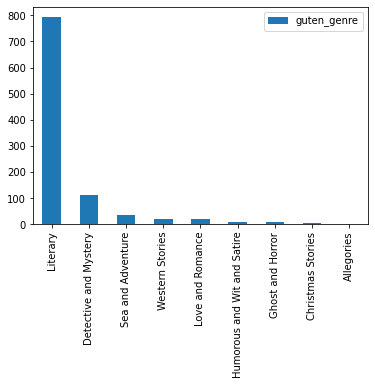
\includegraphics[width = 0.5\textwidth]{Classimbalance.png}
\caption{\label{fig:frog}Genre category and count}
\end{figure}

\section{Data Set}
\justify
The Gutenberg 19th century English Fiction Dataset is a subset of books that belong to the 19th Century English Fiction. \newline It was generated from Project Gutenberg\footnote[1]{\href{https://www.gutenberg.org/}{Project Gutenberg}}, which consists of over 60,000 eBooks, published in the 19th century. For our Dataset, we were given 1079 html files represented as 1079 books that contain the text   and a csv file that contained names of 996 books with the following columns:
\begin{itemize}
  \item Book Name
  \item Book Id (Key)
  \item Guten Genre
  \item Author Name
\end{itemize}\vspace{1mm}
\newpage \justify We have ignored those (1079-996) 83 extra books, for \newline consistency. We have 9 unique genres in the Guten Genre column, namely: 'Detective and Mystery', 'Literary', 'Western Stories', 'Ghost and Horror', 'Christmas Stories' 'Love and Romance', 'Sea and Adventure', 'Allegories', 'Humorous and Wit and Satire' to work with and solve the Genre Classification problem, posed to us. Therefore, Guten Genre will be our target attribute.
We have noticed class imbalance in our dataset, depicted in Fig.1. Although, there are no missing values, for any of the above mentioned columns. For the books, the 'Literary' genre, has the majority count of 794 and 'Allegories' has the least count of 2. These are the initial observations of the dataset.

\section{Concept}
\subsection{Naive Bayes:}
\justify One of the most commonly used algorithm for text classification. It is based on conditional probabilities of the concurrences of a feature and respective label. We have used the model with features extracted in multiple techniques. Bag of words is one of such techniques used. We used the performances of the model features extracted from ‘bag of words’, as a baseline to compare other feature vectors with. We have trained the model individually using ‘bag of words’, ‘tf-idf’ and hand crafted features.
\subsection{Multinomial Naive Bayes:}
\justify In this variation of Bayes algorithms, the term (words) frequency is also taken into account in training. The only difference between the Naive Bayes and Multinomial Naive Bayes is the difference in distribution of feature assumes. Naive Bayes assumes binomial distribution (Hence, naive), while Multinomial assumes Multinomial distribution. Features generated using ‘bag of words’, ‘tf-idf’ and hand crafted features will be used to train the model.
\subsection{Multi Layered Perceptrons:}
\justify Another traditional text classification machine learning model, MLPs, they are simplistic in nature compared to its deep learning\cite{Worsham2018} counterparts. The input will be ‘bag of words’ and ‘tf-idf’. This is one of our baseline model. 
\subsection{Linear SVM:}
\justify Under the assumption that most of the text classification problems are linearly separable we implement linear SVM. The features extraction techniques would be bag of words and handcrafted features. There will be more about the hand crafted features in the later sections. The advantages of using linear SVM is SVMs are fast in general and require lesser computation power compared to deep learning models, since fewer parameters to learn, linear kernels are especially faster compared to other kernels. 
\subsection{CNN:}
\justify We implemented a CNN \cite{Huang2017} deep learning model, where it can be used to automatically generate complex features which can better classify the books. The convolution layers are followed by max pooling layers to prevent learnable parameters count from blowing up retaining the information. This is followed by a fully connected MLP with the 9 nodes representing the genres.
\subsection{Feature extraction:}
\subsubsection{Bag of Words:}
\justify We used the bag of words for of representation of the documents. The purpose of this feature extraction technique is to use it as a baseline\cite{Pieters2018} for comparison with the other forms of features.
\vspace{1mm}
\subsubsection{Term frequency-Inverse document frequency:}
\justify Using this technique to measure the importance of a term in a document. This done by multiplying the how many time the term appears with inverse of its frequency across all the documents. We can choose the top k number of terms which define the document which we can add to the features.
\vspace{1mm}
\subsubsection{Data Preprocessing:}
\justify Basic preprocessing is done to remove the noise from the text dataset and make the data predictable and analyzable. 
\begin{itemize}
    \item Lowercase
    \item Tokenization
    \item Stopword removal
    \item Stemming
    \item numbers and special characters removal
\end{itemize}
\vspace{1mm}
\subsubsection{Hand crafted features:}
\justify The features are hand crafted \cite{Polley,Polleya} to catch the essence of the semantic information.During the extraction of features using Tf-idf and BOW, the semantic information is completely lost. Only statistical information remains. For a task like genre identification it is important to maintain the semantic information. The features below represent better semantic information.
\begin{itemize}
    \item Lexical richness
    \item Word count
    \item Word density
    \item Punctuation count
\end{itemize}

\justify \subsubsubsection{Lexical richness:} 
This feature represents the score computed by ratio of unique lexical items and the total number of words in the document. For every book this unique score is a feature. fig.1 shows the distribution of lexical richness score across the dataset.
\begin{figure}
    \centering
    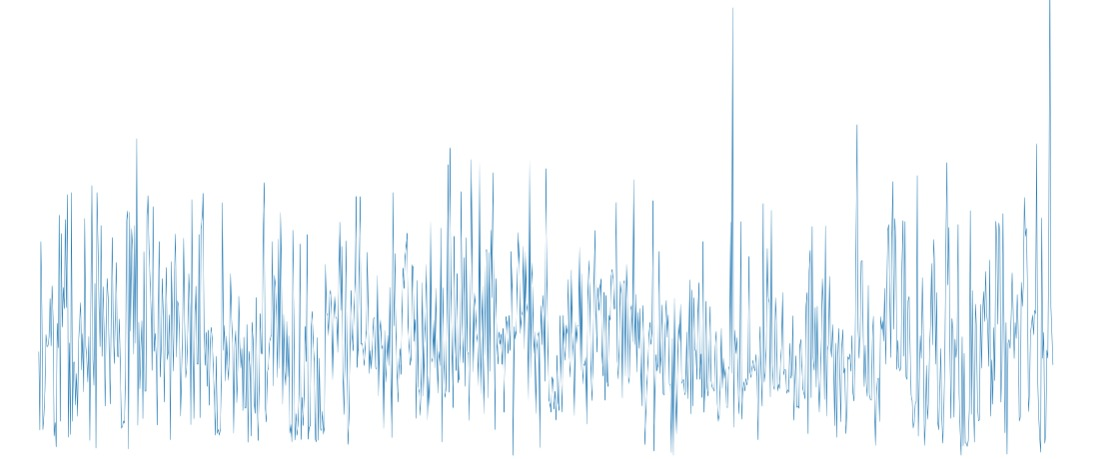
\includegraphics[width=7cm]{lexical_richness}
    \caption{Lexical richness across the entire dataset}
    \label{fig:galaxy}
\end{figure}

\justify \subsubsubsection{Word count:}
The Word count represents the total number of words in every document. 


\justify \subsubsubsection{Inverse word density:}
Inverse Word density represents Word count divided by Character count.

\justify \subsubsubsection{Punctuation count:}
The Punctuation count represents the count of the punctuation in every document.




\section{Implementation}
\vspace{1mm}
\justify We have implemented the said models using the tools, mentioned in  table \ref{table:1}.
\begin{wrapfigure}


\begin{table}[h!]
\centering
\begin{tabular}{ |p{0.5cm}||p{3cm}|p{1.2cm}|p{4cm}|  }
 \hline
 \multicolumn{4}{|c|}{Tools and Libraries} \\
 \hline
 Sr.no. & Library Name or Tool  & Version & Purpose\\
 \hline
 1. & Codecs                    &   1.3.2 &   To parse content from an HTML file       \\
 \hline
 2. & Natural Language Toolkit  & 3.2.5   &    To tokenize and stem words      \\
 \hline
 3. & Pandas                    & 1.0.5    &  Data analysis and manipulation        \\
 \hline
 4. & Numpy                     &  1.18.5  &   To process arrays         \\
 \hline
 5. & Scikit-learn              & 0.22.2.post1   & a) To vectorize text content.
(TF-IDF/TF)
\newline b) To import classifiers.
\newline c) To split the data in K
folds.
\newline d) To find the evaluation
metrics         \\
 \hline
 6. & Google Colab              &  ----  & Exploit faster processing speed \\
 \hline
 7. & keras                       &  2.3.1  & for deep learning model layers                  \\
 \hline
 8. &  Pickle                   & 4.0   &  Used to serialize and de-serialize Python object structures, also called marshalling or flattening.  \\
 \hline
 9. &  Tensorflow                         & 2.2.0   &  for deep learning models              \\
 \hline
\end{tabular}
\vspace{1mm}
\caption{Tools and Libraries}
\label{table:1}
\end{table}
\end{wrapfigure}
\justify
The Source code consists of data preprocessing, and use of different models like Gaussian Naive Bayes, Multinomial Naive Bayes, Bernoulli naive Bayes, Linear Support Vector Machine from Scikit-learn library and Mutli-Layer Perceptron and Convolutional Neural Network from keras library. You can find below a couple of snippets from the source code. We concatenated the hand features with the Tf-idf vectors and feed the model for only machine learning techniques. We are using MLP and Convulational Neural Networks in Deep Learning portion for the classification task.



\vspace{2mm}
\section{Evaluation}
\vspace{1mm}
\subsection{Evaluation Metrics:}
\justify

We used Scikit-learn for training data and test data split.
\newline
75 percentage of corpus data used as training set, and 25 percentage as test set.
We used 1000 iterations for traditional models and 20 epochs for deep learning metrics of batch size 32.
We used 3 metrics for model evaluation.
Accuracy, Precision, and F1-score.
We are getting around 78 percentage accuracy on different models. All models are performing better.
The difference between training accuracy and testing accuracy is very low, thus we can understand model is generalizing well.
Overall Problem goal is accomplished. Although we can get better by tweaking the model, still we are getting good results.


\newpage
\begin{table}[t]
\centering
\begin{tabular}{ |p{4cm}||p{4cm}|p{4cm}|p{4cm}|  }
 \hline
 \multicolumn{4}{|c|}{Evaluation Metrics} \\
 \hline
 Model & Accuracy  & F1-Score & Precision\\
 \hline
 Gaussian Naive Bayes &       0.787              &  0.7692  & 0.7545         \\
 \hline
 Multinomial Naive Bayes & 0.811 & 0.726  & 0.658          \\
 \hline
 Bernoulli Naive Bayes &       0.6746             & 0.7192   &   0.808       \\
 \hline
 Linear Support Vector machine &      0.8514              & 0.8081   &     0.823       \\
 \hline
 Multi Layer Perceptron &      0.8795         & ---- & ---- \\
 \hline
 Convolutional Neural Network & 0.7871 &  ----  & ---- \\
 \hline
\end{tabular}
\vspace{1mm}
\caption{Evaluation Metrics}
\label{table:2}
\end{table}


\section{Conclusion}
\vspace{1mm}
\justify
Challenges: Reading and storing the data from HTML files all at once is complicated task, since it is eating all the memory. When we tried to use Entity Recognition for feature extraction, the run time is high for the whole corpus.
Similarly, also to retrieve Parts-of-speech tagging, and porter stemming the run time is high.
Our results can be considered as base model results and can be used to perform improvements and hyper parameter tuning.


\vspace{1mm}
\justify
Results: We could extract more topic specific hand crafted features, by fine tuning the model.
We could Also augment the data, instead of considering a single documents as multiple documents, to remove class imbalance.





































\medskip

\printbibliography
\end{document}
